% ==============================================
% CFD Tutorial Template: OpenFOAM Terminal Basics
% Class: scrartcl (KOMA-Script) - optimized for tutorials
% Content: pitzDaily with simpleFoam
% ==============================================

\documentclass[
parskip=half,      % Space between paragraphs (better for steps)
DIV=12,            % Optimal margins for readability
headings=normal,   % Professional heading sizes
fontsize=11pt,     % Slightly larger for screen reading
english            % Language setting
]{scrartcl}

\input{../preamble.tex}
\usetikzlibrary{intersections}

% ========== DOCUMENT START ==========
\begin{document}
	
	% ========== TITLE PAGE ==========
	\title{Tutorial \#5: 3D Y-Pipe with FreeCAD}
	\subtitle{Incompressible Steady Flow: 3D Y-Pipe with simpleFOAM in FreeCAD}
	\subject{Open Source CFD }
	\author{Robert Castilla \\ Department of Fluid Mechanics}
	\date{2025-26 \\ Version 1.0}
	\publishers{Learning Objectives:
		\begin{itemize}
			\item Set up a complete CFD case using FreeCAD and CfdOF workbench
			\item Define boundary conditions visually in the GUI
			\item Generate mesh automatically with snappyHexMesh
			\item Run simpleFoam directly from FreeCAD
			\item Post-process results using ParaView integration
			\item Compare GUI vs terminal workflows (Tutorial \#4)
		\end{itemize}}
	
	\maketitle
	
	% ========== ABSTRACT ==========
	\begin{abstract}
		This tutorial shows the work flow for the simulation of a 3D Y-shaped
		pipe geometry with FreeCAD and the CfdOf workbench.
		The geometry generated in Tutorial \#4 will be reused. Instead of 
		editing manually the dictionaries, in this case all will be done with the GUI. It is more efficient and reduces the risk of typographic mistakes. On the other side, a graphical interface, that often is not available in large computers, is needed.
	\end{abstract}
	
	\tableofcontents
	\newpage
	
	
	\section{Opening the Geometry in FreeCAD}
	
	\begin{enumerate}
		\item \textbf{Launch FreeCAD} from the terminal or applications menu:

		
		\item \textbf{Open the Y-pipe geometry}:
		\begin{itemize}
			\item Go to \texttt{File $\rightarrow$ Open}
			\item Navigate to your Tutorial \#4 folder
			\item Select \texttt{Ypipe.FCStd}
			\item Click \texttt{Open}
		\end{itemize}
		
		\begin{figure}[h]
			\centering
			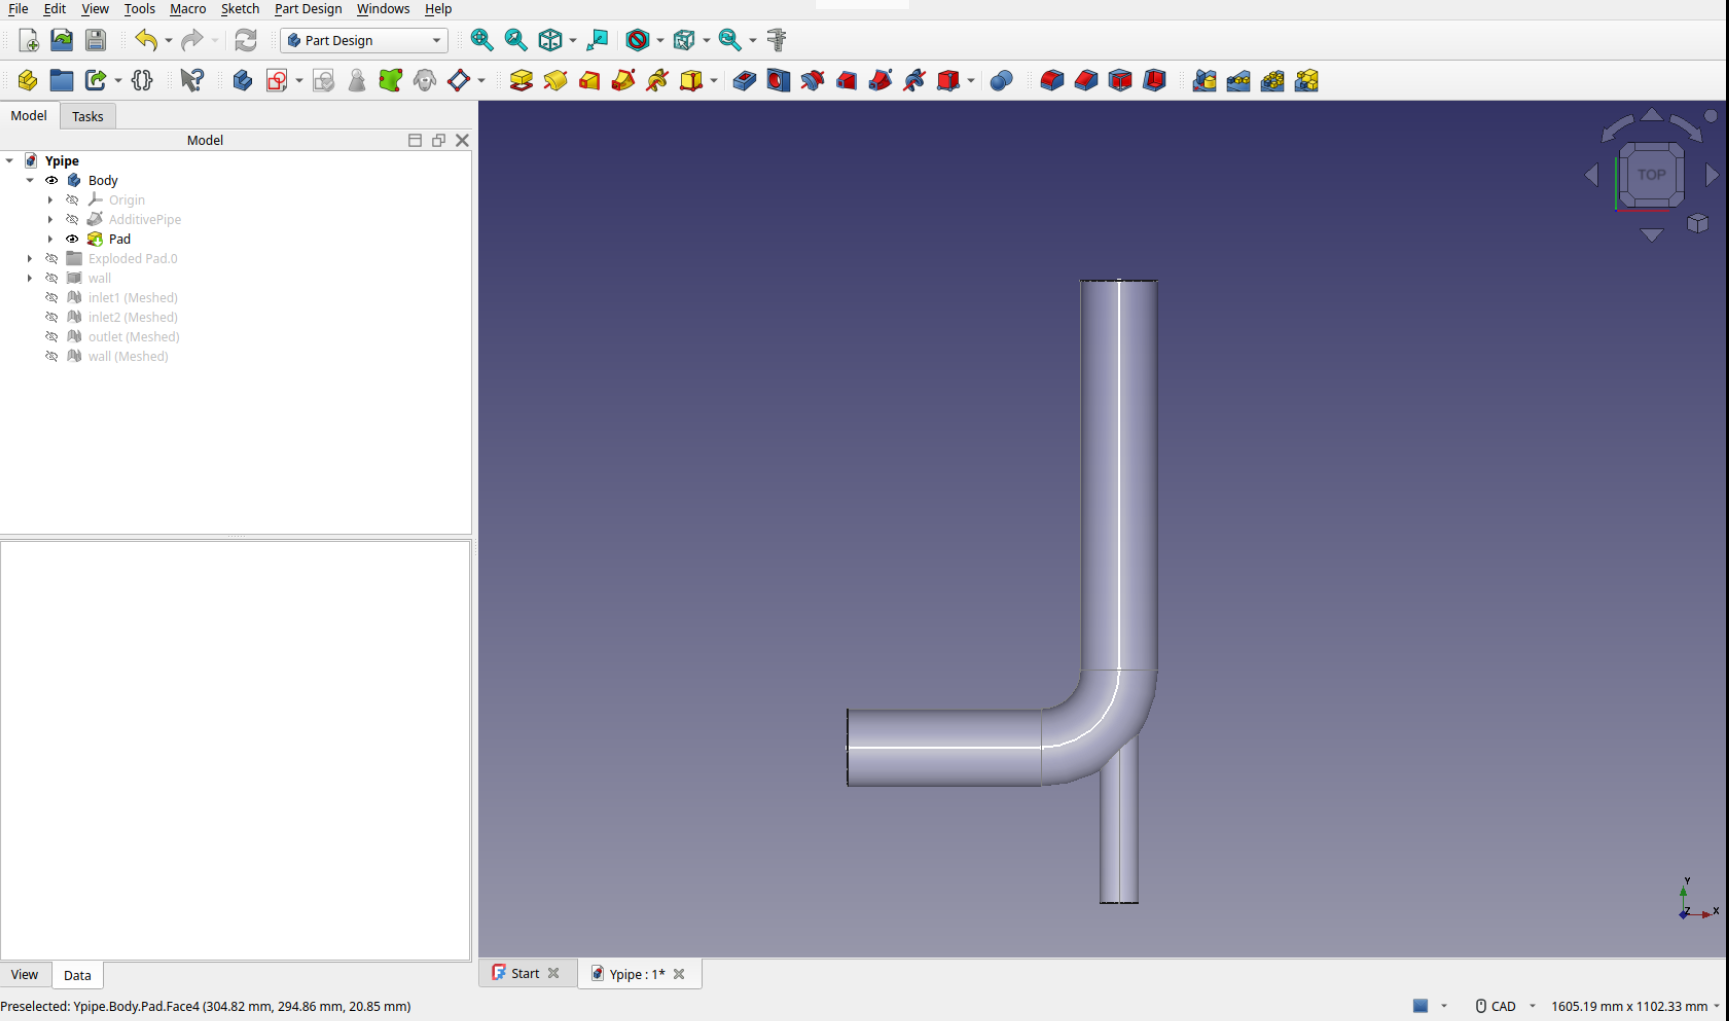
\includegraphics[width=0.8\linewidth]{open_file}
			\caption{Opening the Y-pipe geometry}
			\label{fig:open}
		\end{figure}
		
		\item \textbf{Verify the geometry}:
		\begin{itemize}
			\item The model should appear in the 3D view
			\item The tree view should show the \texttt{Body} with all features
			\item Rotate and zoom to inspect all parts
		\end{itemize}
		
		\tip{If you don't have the geometry file, follow the geometry creation steps from Tutorial \#4, Sections 2.1-2.2.}
		
	\end{enumerate}
	 
	 \section{Setting Up the CFD Analysis}
	 
	 \subsection{Activating CfdOF Workbench}
	 
	 \begin{enumerate}
	 	\item \textbf{Switch to CfdOF workbench}:
	 	\begin{itemize}
	 		\item From the workbench dropdown, select \textbf{CfdOF}
	 	\end{itemize}
	 	
	 	
	 \item \textbf{Change output directory}
	 \begin{itemize}
	 	\item Select the menu \texttt{CfdOf $\rightarrow$ Open preferences}
	 	\item Change the \texttt{default output directory} to your folder for the Tutorial \#5.
	 \end{itemize}
	 
	 	\begin{figure}[h]
	 		\centering
	 		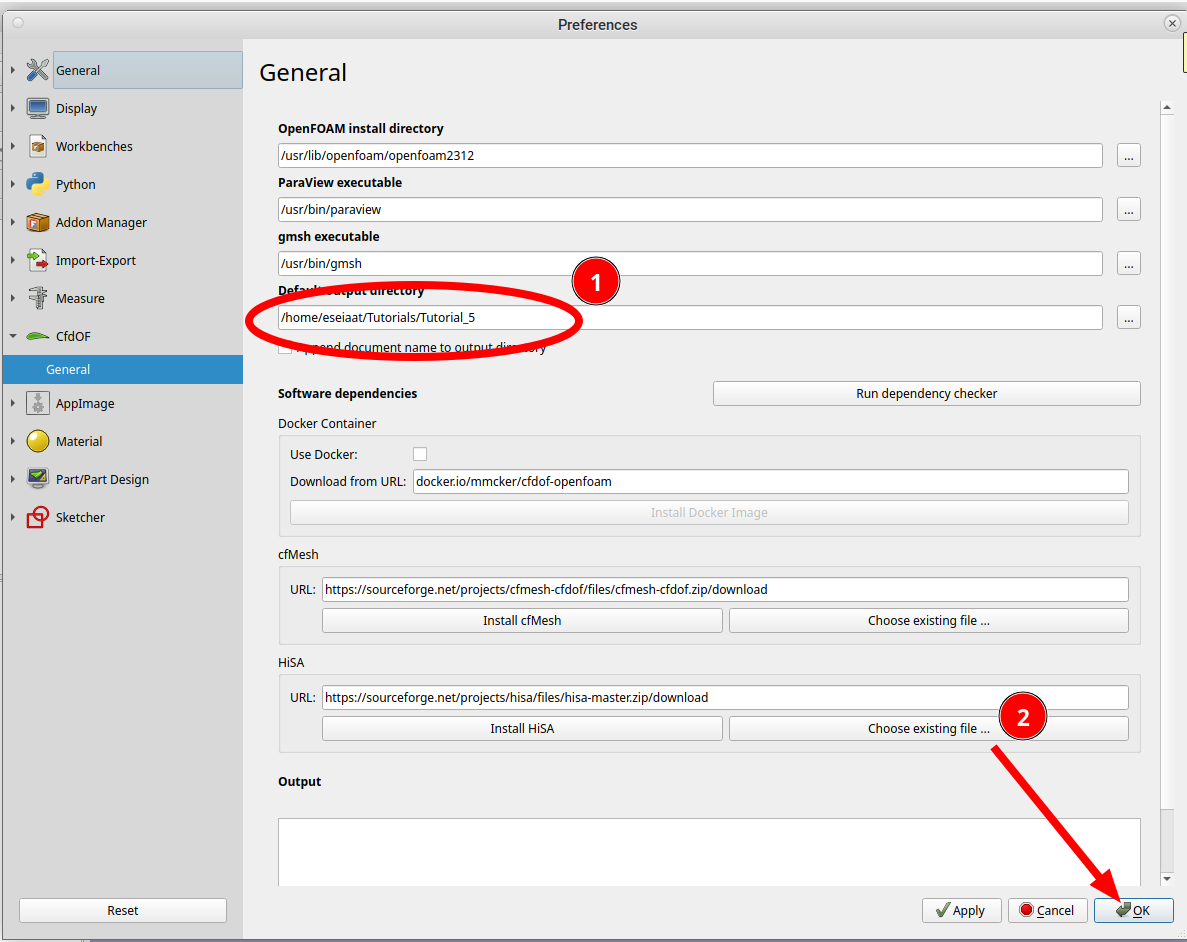
\includegraphics[width=0.5\linewidth]{select_folder}
	 		\caption{Selecting of output directory}
	 		\label{fig:cfdof}
	 	\end{figure}
	 	
	 	\item \textbf{Create a new analysis}:
	 	\begin{itemize}
	 		\item Click the \textbf{Analysis container} button in the toolbar
	 		\item A new \texttt{CfdAnalysis} object appears in the tree
	 	\end{itemize}
	 \end{enumerate}
	 
	 \subsection{Defining the Simulation}
	 
	 \begin{enumerate}
	 	
	 	\item \textbf{Set physics models}:
	 	\begin{itemize}
	 		\item Click on \texttt{Select models} button
	 		\item In the Tasks panel, set:
	 		\begin{itemize}
	 			\item \texttt{Flow type}: \texttt{Incompressible}
	 			\item \texttt{Time}: \texttt{Steady}
	 			\item \texttt{Turbulence model}: \texttt{RANS k-omega SST}
	 		\end{itemize}
	 	\end{itemize}
	 	
	 	\begin{figure}[h]
	 		\centering
	 		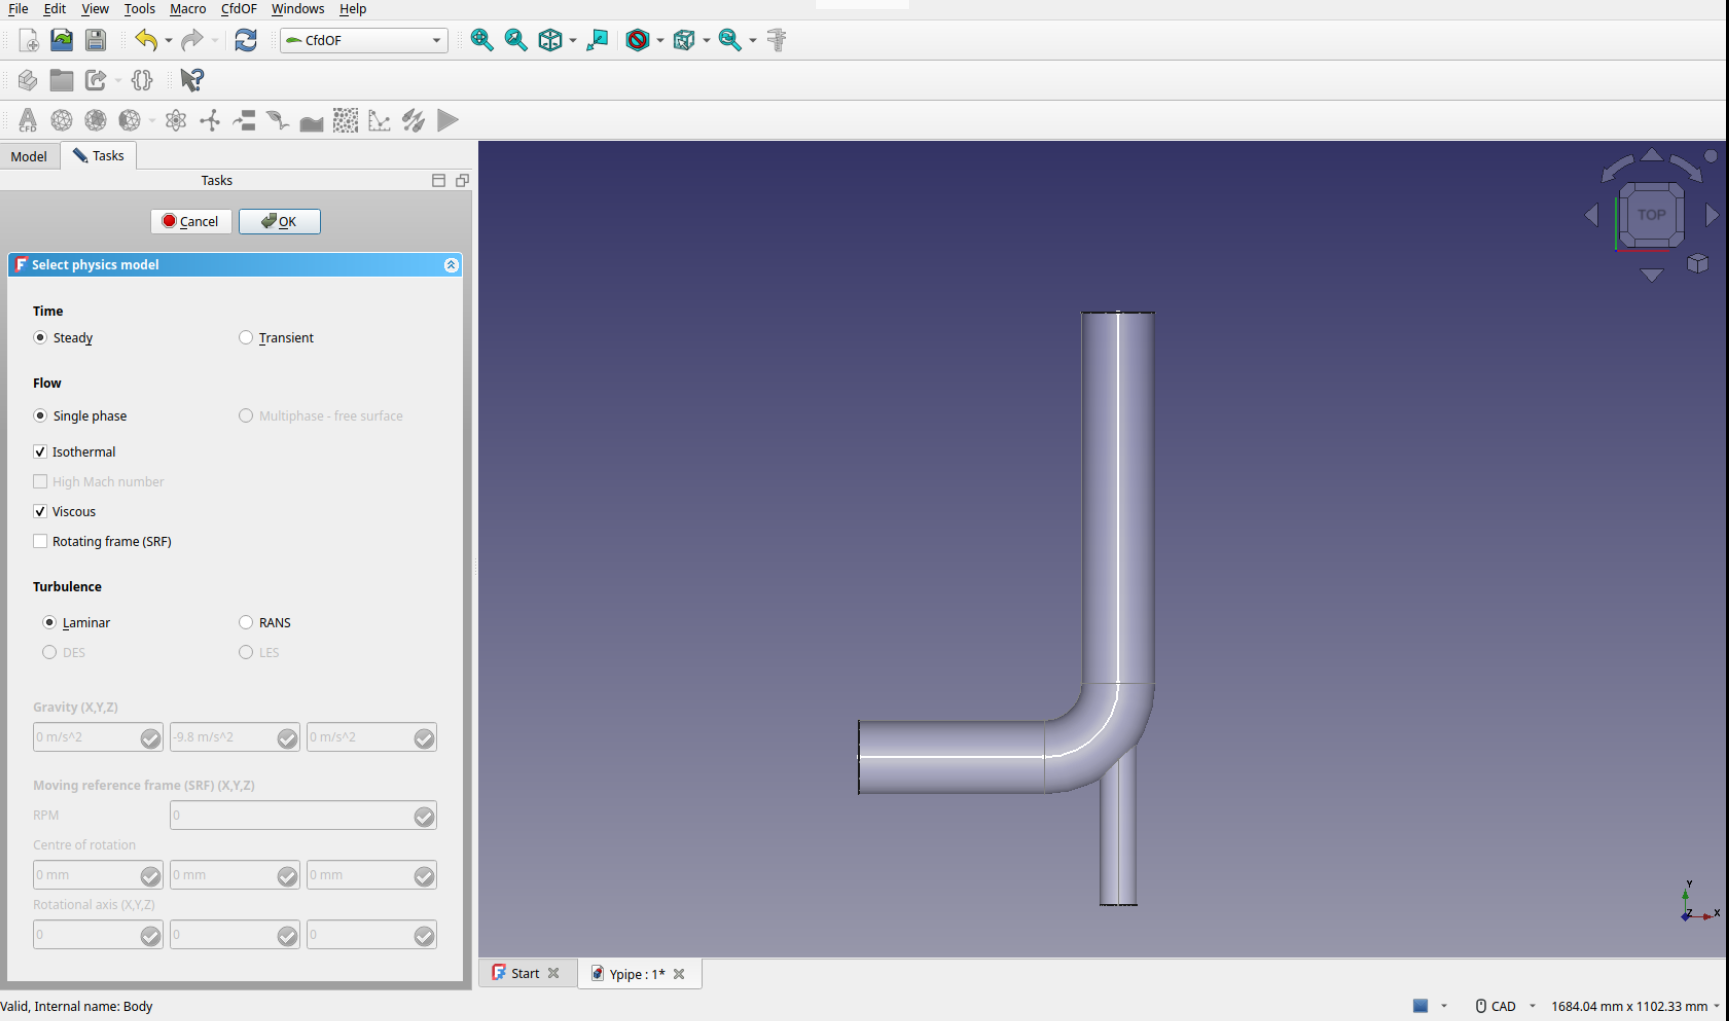
\includegraphics[width=0.7\linewidth]{models}
	 		\caption{Physics models}
	 		\label{fig:models}
	 	\end{figure}
	 	
	 	\item \textbf{Select fluid material}:
	 	\begin{itemize}
	 		\item Click \textbf{Add fluid properties} button
	 		\item Choose \texttt{Water} from the library
	 		\item Verify properties: $\rho = \qty{1000}{kg/m^3}$, $\nu = \qty{e-3}{Pa\cdot s}$
	 	\end{itemize}
	 \end{enumerate}
	 
	 \section{Defining Boundary Conditions}
	 
	 \subsection{Identifying Boundary Faces}
	 
	 The Y-pipe has four distinct boundary regions:
	 \begin{itemize}
	 	\item \textbf{inlet1}: Secondary inlet (horizontal branch)
	 	\item \textbf{inlet2}: Primary inlet (vertical pipe)
	 	\item \textbf{outlet}: Pipe outlet
	 	\item \textbf{wall}: All remaining surfaces
	 \end{itemize}
	 
	 \subsection{Creating Boundary Conditions}
	 
	 \begin{enumerate}
	 	\item \textbf{Add inlet2}:
	 	\begin{itemize}
	 		\item Select \texttt{inlet2} face (secondary inlet). It will become green.
	 		\item Click \textbf{Fluid boundary} button. It will become blue
	 		\item \texttt{Type}: \texttt{Inlet, Uniform velocity }
	 		\item \texttt{Velocity}: \texttt{(0 4 0)} m/s (vertical direction)
	 		\item \texttt{Pressure}: \texttt{0} Pa (relative pressure)
	 		\item Click \texttt{OK}
	 		\item \texttt{Turbulence specification: Intensity \& Length Scale}
	 		\begin{itemize}
	 			\item \texttt{Intensity (I)}: 5\%
	 			\item \texttt{Length Scale (l)}: \qty{1.4}{mm}
	 		\end{itemize}
	 		\item Rename it as \texttt{inletSecondary}
	 	\end{itemize}
	 	
	 		\tip{\texttt{CfdOf} automatically calculates $k$ and $\omega$ from these parameters using standard formulas: 
	 		$k = \frac{3}{2}(UI)^2$, $\omega = \frac{\sqrt{k}}{C_\mu^{1/4}L}$ where $C_\mu = 0.09$ and $L$ is the mixing length scale.}
	 	
	 		 	\begin{figure}[h]
	 		\centering
	 		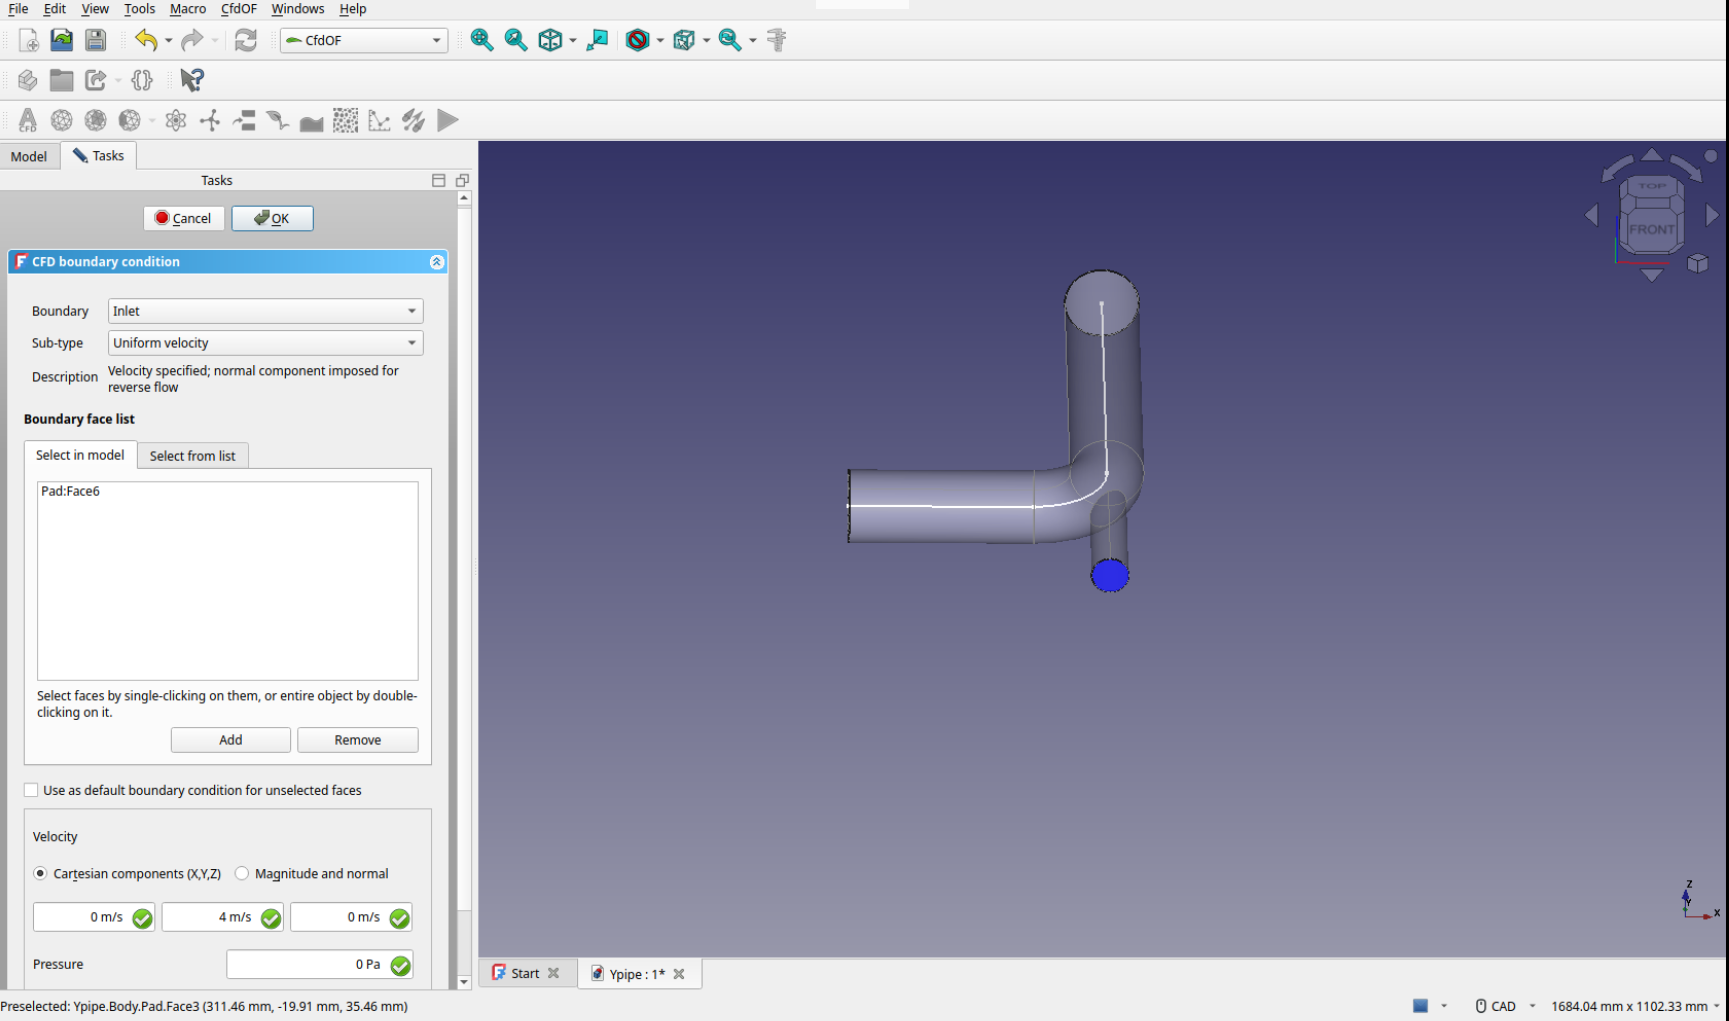
\includegraphics[width=0.7\linewidth]{boundary_inlet}
	 		\caption{Setting inlet boundary conditions}
	 		\label{fig:boundary}
	 	\end{figure}
	 	
	 	\item \textbf{Add inlet1}:
	 	\begin{itemize}
	 		\item Repeat the same steps as with \texttt{inlet2}
	 		\item \texttt{Type}: \texttt{inlet, Total pressure}
	 		\item Set \texttt{Pressure} : \qty{0}{Pa}
	 		\item Same turbulence specification as in \texttt{inlet2}
	 		\item Rename it as \texttt{inletMain}
	 	\end{itemize}
	 	

	 	
	 	\item \textbf{Add outlet}:
	 	\begin{itemize}
	 		\item Repeat the same steps
	 		\item \texttt{Type}: \texttt{outlet, Static pressure}
	 		\item \texttt{Pressure}: \texttt{0 Pa} (static)
	 		\item Leave the default name (\texttt{outlet} is not allowed because there is already an element in the tree with this name)
	 	\end{itemize}
	 	
	 	\item \textbf{Add walls}:
	 	\begin{itemize}
	 		\item Select all remaining faces (use Ctrl+click for multiple
	 		selection)
	 		\item \texttt{Type}: \texttt{wall}
	 		\item \texttt{Name}: \texttt{walls}
	 	\end{itemize}
	 	
	 	\item \textbf{Verify all boundaries}:
	 	\begin{itemize}
	 		\item The tree should show four boundary conditions
	 		\item Each should have a distinct color in the 3D view
	 	\end{itemize}
	 	
	 	\begin{figure}[h]
	 		\centering
	 		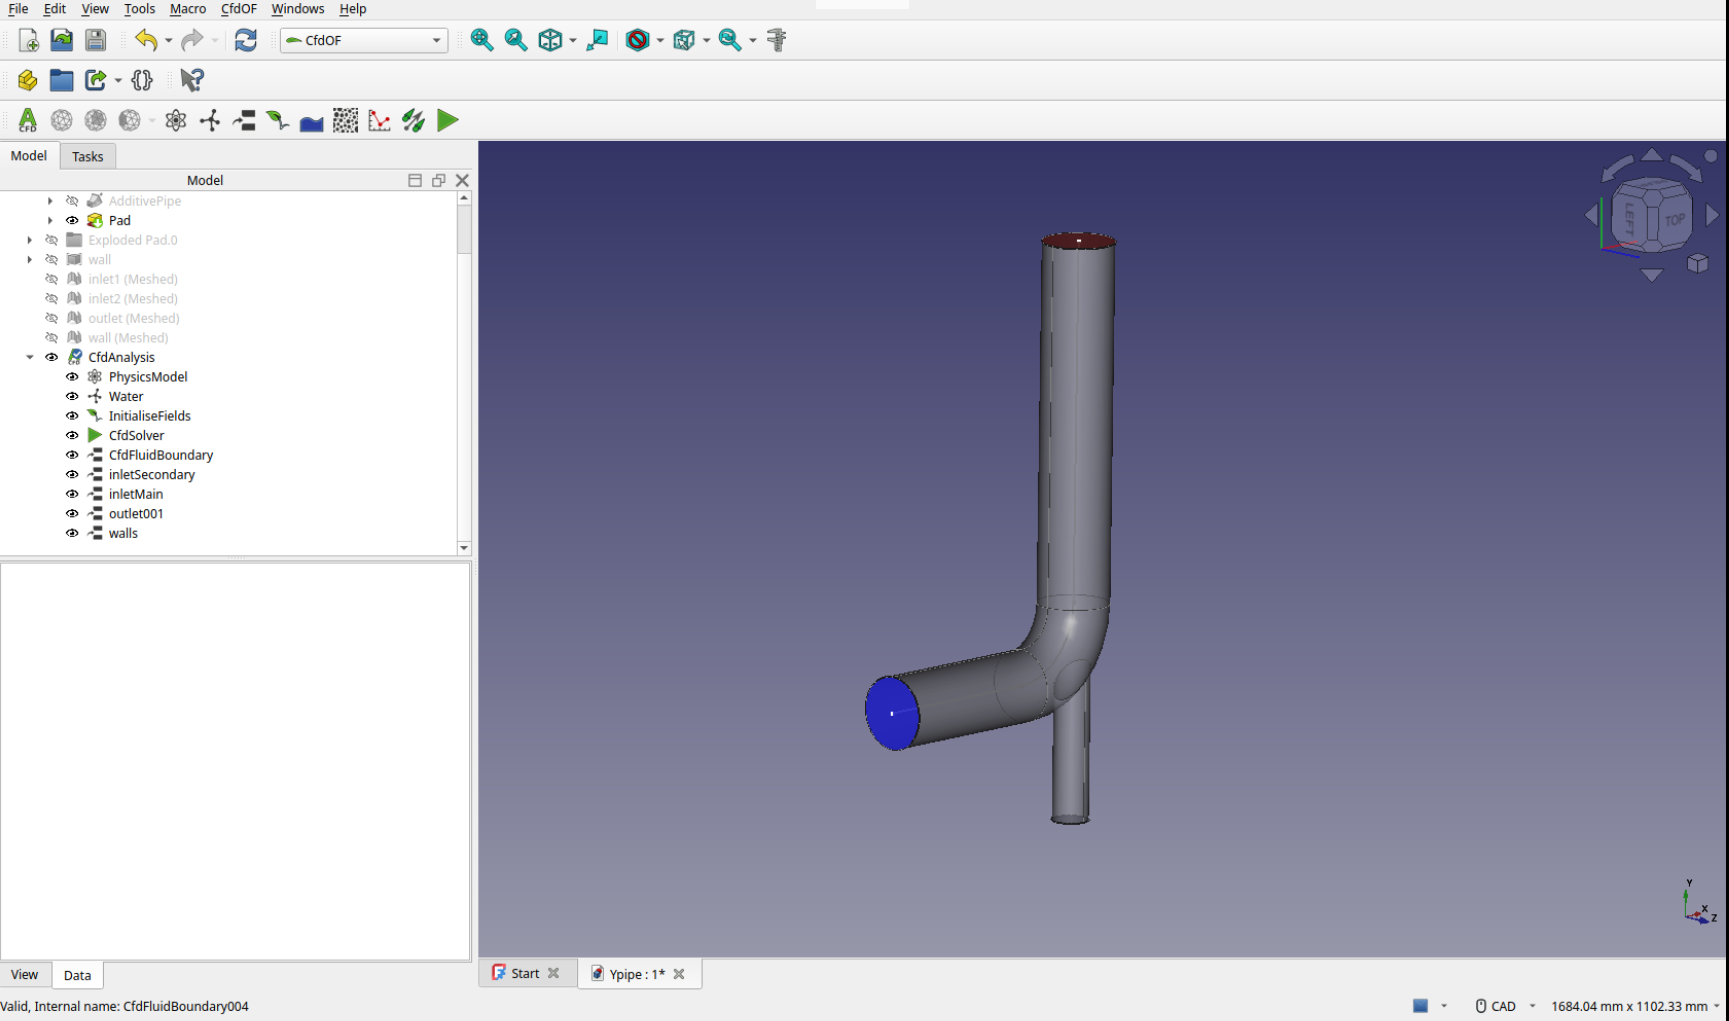
\includegraphics[width=0.7\linewidth]{boundaries}
	 		\caption{Completed boundary conditions}
	 		\label{fig:boundaries}
	 	\end{figure}
	 \end{enumerate}
	
	
	

		
\end{document}